Once assigned to the GIRAF project the papers written the previous year are distributed amongst the groups in order to accumulate some knowledge of what they did, what they may not have had time to do,  how they worked and most importantly the evaluation thereof.
These papers provide a basis from which organisational tasks can be identified and assigned to groups involved in the development of GIRAF for this semester.

\section{Development Method and Organisational Tools}
The first meeting serves to address introduction of the most immediate organisational aspects such as version control, communication, development method, meetings and significant areas of responsibility.
For this meeting each group provides a list of the most significant pros and cons identified in each paper read, three papers per group in order to assure each paper was read at least twice.
These pros and cons are used in consideration of development method and organisational tools.

\subsubsection*{Development Method}
All previous semesters of the GIRAF project used the agile development method scrum.
Scrum is an agile development method, which uses small teams with small sprints. 
A product back-log is kept which contain the tasks which need to be made for the project. 
When a sprint starts some tasks from the product back-log are transferred to a sprint back-log and theses tasks will then be completed before the end of the sprint.
Scrum uses a daily meeting which is called a daily scrum, which get everyone in the group up to speed on what everyone is working on, and if any problems are occurring. 
A burndown chart is used to keep track of the progress for each sprint. 
Every task is time estimated, and so all tasks for the sprint give a total worktime, and each time a task is completed, the burndown chart is updated so progress can easily be estimated.

A scrum board is also used, which keeps track the sprint back-log, which tasks are being worked on, which are ready to be reviewed, which are done, and which have not been started yet.
A couple of roles are normal in scrum, the product owner and the scrum master.
The product owner is the group member who controls the product back-log, it is their job to understand what the customer wants, and therefore how to prioritize the different tasks on the back-log.
The scrum master is the person who works to ensure that the development team uses scrum correctly, and helping the product owner organizing the product back-log.
For more information on scrum see the Scrum Alliance guide. \cite{scrum}
\todo[inline]{Skal vi have mere om scrum eller er dette tilstrækkeligt? - Soren}

\bigskip
The multi-project from last year used a method called scrum of scrums, which tries to take some of the principles from scrum and apply it on a larger group.
This works by having multiple groups, which all do scrum, and then having ambassadors from every group meet and do the scrum meetings. 
Every group will perform a daily scrum as usual, and the multi-group will perfrom a scrum meeting answering the same questions as one would at daily scrum, but instead it is just the ambassadors from each group at this scrum meeting, which then speak on the group's behalf.
The questions are as follows:

\begin{itemize}
	\item What did you do yesterday? 
	\item What will you do today?
	\item What obstacles are in your way or slowing you down?
\end{itemize}

These questions suggest that the meeting weill be held daily, though it is recommended to have the scrum of scrums two to three times a week instead.
Last year the students had a meeting two times a week, and some groups complained that this was too much, and this is agreed upon in the multi-project, so a single meeting once a week is suggested instead.
The recommendation of two to three times a week is based upon how scrum of scrum is used in the private sector, but as we are students we are not working on the GIRAF project all the time, we have courses which also require work, which leaves us with less time to work on the GIRAF project. 
These reasons seemed like valid arguments for having the scrum of scrum once a week.

The scrum of scrum meeting organisation can be seen on \myref{fig:scrumofscrum}.

\begin{figure}
\centering
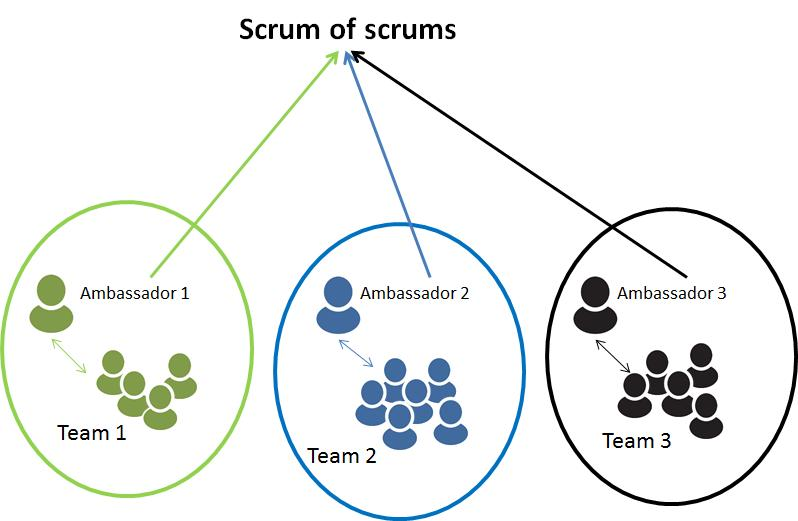
\includegraphics[scale=0.4]{figures/scrumofscrum.png}
\caption{The structure of scrum of scrum.}
\label{fig:scrumofscrum}
\end{figure}

For the scrum of scrum a single product back-log with tasks will also be made, and each group in the multi-project will then take tasks or user stories from this back-log and put these on their own internally kept sprint back-log.

The roles of the product owner and scrum master will instead be areas of responsibility of certaing groups in the multi-project, which will be explained next.

\subsubsection*{Areas of Responsibility}
Areas of responsibility are organisational and technical aspects of development that may require attention but are not necessarily directly linked to the software itself.
The use of Scrum dictates that a project owner and a Scrum master exists, as the Scrum is composed of groups, these roles will be assigned to groups as areas of responsibility.
Furthermore the servers, the database and Jenkins, the automated build, has, according to the papers read, often caused trouble so these will also serve as areas of responsibility.
According to previous papers these groups also have a great deal of interaction, in order to reduce the time spent explaining the issue to other groups these areas will all be handled by the same group, as it happens all the areas is far too big a workload for a single group, thus two groups share these responsibilities.
From the previous papers it is evident that their work flow did not include a formal or even uniform way of documentation or even code.
As such documentation and unit/integration testing are also established as areas of responsibility, documentation being the one we are responsible for.
Further areas of responsibility are derived largely from suggestions or positive feedback from the read papers, these include graphics, usability tests, security and social events/HR
\info[inline]{jeg oververjer at stille alle op som punktform og forklare dem men ved ikke om det bliver for meget?}

\subsubsection*{Development and Organisational Tools}
Redline -> Phrabricator
Redline Forum -> Slack
Android Studio -> target/minimum API(Maybe???)
Google Docs(Meeting Summary)
